%============================================================
% RUNNER: PROPOSAL PROYEK AKHIR
% Output : output/proposal/Proposal_PA_*.pdf
%
% Isi:
%   - Cover Proposal PA (putih, logo grayscale)
%   - Bab 1 (Pendahuluan) s.d. Bab 3 (Desain Sistem)
%   - Daftar Pustaka
%
% Format: single-sided, margin 2.5/3.0cm (Panduan PASPE-2022)
%============================================================

\documentclass[12pt, a4paper, oneside, fleqn]{report}


% ============================================================
% KONFIGURASI OPSIONAL: Uncomment untuk mengaktifkan
% ============================================================
% Front matter (default semua off):
% \showabstraktrue         % Tampilkan Abstrak Bahasa Indonesia
% \showabstracttrue        % Tampilkan Abstract Bahasa Inggris
% \showdaftarisitrue       % Tampilkan Daftar Isi
% \showdaftargambartrue    % Tampilkan Daftar Gambar
% \showdaftartabeltrue     % Tampilkan Daftar Tabel
%
% Paksa setiap konten baru ke halaman ganjil (default off):
% \showforceoddpagetrue
% ============================================================

% Konfigurasi (urutan penting)
%============================================================
% VARIABEL IDENTITAS DOKUMEN
% Edit bagian ini sesuai dengan data proyek akhir Anda.
% File ini di-input pertama kali agar semua file lain
% dapat mereferensikan variabel-variabel berikut.
%============================================================

% ── Identitas Mahasiswa ──────────────────────────────────────
\newcommand{\NamaMahasiswa}{Jhiven Agnar Fuad}
\newcommand{\NRP}{3122600052}

% ── Judul Proyek Akhir ───────────────────────────────────────
% Tulis judul dengan kapitalisasi biasa; \MakeUppercase
% diterapkan secara otomatis di tempat yang membutuhkannya.
\newcommand{\JudulPA}{Lorem ipsum dolor sit amet, consectetur adipiscing elit.
  Nam sed aliquam odio, eu congue ex. Aenean aliquet non dui a interdum. Sed nec
  metus
}

% ── Dosen Pembimbing (sertakan gelar akademis) ───────────────
\newcommand{\NamaPembimbingSatu}{Umi Sa'adah, S.Kom., M.Kom.}
\newcommand{\NIPPembimbingSatu}{197404162000032003}
\newcommand{\NamaPembimbingDua}{Dr. Tita Karlita, S.Kom., M.Kom.}
\newcommand{\NIPPembimbingDua}{197910142002122002}

% ── Dosen Penguji (sertakan gelar akademis) ──────────────────
\newcommand{\NamaPengujiSatu}{Nama Lengkap dan Gelar}
\newcommand{\NIPPengujiSatu}{xxxxxxxxxxxxxxx}
\newcommand{\NamaPengujiDua}{Nama Lengkap dan Gelar}
\newcommand{\NIPPengujiDua}{xxxxxxxxxxxxxxx}

% ── Pembimbing Opsional (Isi salah satu saja, atau kosongkan keduanya) ──
% Isi jika memiliki Dosen Pembimbing ke-3 (Akademik)
\newcommand{\NamaPembimbingTiga}{}
\newcommand{\NIPPembimbingTiga}{}

% Isi jika memiliki Pembimbing dari Industri
\newcommand{\NamaPembimbingIndustri}{Willy Achmat Fauzi, S.ST., M.T.}

% ── Ketua Program Studi (sertakan gelar akademis) ────────────
\newcommand{\NamaKetuaProdi}{Yanuar Risah Prayogi, S.Kom., M.Kom}
\newcommand{\NIPKetuaProdi}{198801062019031009}

% ── Program Studi & Institusi ────────────────────────────────
\newcommand{\NamaProdi}{Teknik Informatika}
\newcommand{\NamaDepartemen}{Departemen Teknik Informatika Dan Komputer}

% ── Gelar yang Diperoleh ─────────────────────────────────────
\newcommand{\GelarLulus}{Sarjana Terapan Komputer (S.T.r.Kom.)}

% ── Tahun Kelulusan ──────────────────────────────────────────
\newcommand{\TahunLulus}{2026}

% ── Tanggal Sidang ───────────────────────────────────────────
% Dipakai di halaman pernyataan. Format: Surabaya, DD Bulan YYYY
\newcommand{\TanggalSidang}{Surabaya, \today}

\input{config/toggles}

% Override toggle SETELAH config/toggles
\proposaltrue
% ── Opsi Front Matter & Layout ─────────────────────────────────
% Secara default dinonaktifkan. Hapus tanda % (uncomment) pada
% baris di bawah ini untuk mengaktifkan fitur yang diinginkan.
% Baca [README.md](README.md) untuk detail selengkapnya.
% \showabstraktrue         % Tampilkan Abstrak Bahasa Indonesia
% \showabstracttrue        % Tampilkan Abstract Bahasa Inggris
% \showkatapengantartrue   % Tampilkan Kata Pengantar
% \showdaftarisitrue       % Tampilkan Daftar Isi
% \showdaftargambartrue    % Tampilkan Daftar Gambar
% \showdaftartabeltrue     % Tampilkan Daftar Tabel
% \showforceoddpagetrue    % Paksa setiap konten baru ke halaman ganjil

\input{config/packages}
%============================================================
% FORMATTING: BASE LAYER (SHARED)
% Aturan yang 100% sama di Proposal, Progres, dan Buku PA.
% Aturan per-dokumen (geometry, spacing) ada di formats/format_*.tex
% yang di-input SETELAH file ini di masing-masing main_*.tex.
%============================================================

% ── Warna Institusi ──────────────────────────────────────────
\definecolor{pensbiru}{RGB}{0, 47, 167}    % Biru PENS (#002FA7)
\definecolor{penskuning}{RGB}{255, 193, 7} % Kuning/emas garis cover

% ── Nonaktifkan Hyphenation (pemenggalan kata) ──────────────
% Mencegah LaTeX memotong kata di akhir baris (mis. "Elek-tronika").
% tolerance=9999 + emergencystretch memberi ruang fleksibel agar
% LaTeX tidak perlu Overfull saat hyphenation dinonaktifkan.
\hyphenpenalty=10000
\exhyphenpenalty=10000
\tolerance=9999
\emergencystretch=3em

% ── Indentasi & Paragraf ─────────────────────────────────────
% \parindent TIDAK diset di sini - tiap dokumen punya nilai sendiri:
%   Buku PA  : 1.27cm (ada di formats/format_buku.tex)
%   Proposal : 0.75cm (ada di formats/format_proposal.tex)
%   Progres  : 0.75cm (ada di formats/format_progres.tex)
\setlength{\parskip}{0pt}

% ── Persamaan Matematika ─────────────────────────────────────
\setlength{\mathindent}{10mm}
\setlength{\abovedisplayskip}{12pt}
\setlength{\belowdisplayskip}{12pt}
\setlength{\abovedisplayshortskip}{12pt}
\setlength{\belowdisplayshortskip}{12pt}

% Nomor persamaan dicetak tebal-miring
\makeatletter
\renewcommand{\tagform@}[1]{\maketag@@@{\bfseries\itshape(#1)\@@italiccorr}}
\makeatother

% ── Format Judul Bab ─────────────────────────────────────────
\titleformat{\chapter}[display]
{\centering\fontsize{14}{17}\bfseries}
{BAB \thechapter}
{0pt}
{}
\titlespacing*{\chapter}{0pt}{-20pt}{18pt}

% ── Auto-selaraskan indentasi paragraf pertama dengan huruf judul (bukan nomor) ──
\newsavebox{\KotakLabelJudul}
\newdimen\LebarLabelJudul
\newcommand{\SelaraskanIndentAsli}[1]{%
  \sbox{\KotakLabelJudul}{#1}%
  \global\LebarLabelJudul=\wd\KotakLabelJudul
  \global\advance\LebarLabelJudul by 1em
  \xdef\ParindentAsliTersimpan{\the\parindent}%
  \global\parindent=\LebarLabelJudul
  \global\everypar{\parindent=\ParindentAsliTersimpan\relax\global\everypar{}}%
}

% ── Format Judul Subbab (Section) ────────────────────────────
\titleformat{\section}
{\fontsize{14}{17}\bfseries}
{\thesection}
{1em}
{}
[\SelaraskanIndentAsli{\thesection}]
\titlespacing*{\section}{0pt}{15pt}{0pt}

% ── Format Judul Sub-subbab (Subsection) ─────────────────────
\titleformat{\subsection}
{\fontsize{12}{14}\bfseries}
{\thesubsection}
{1em}
{}
[\SelaraskanIndentAsli{\thesubsection}]
\titlespacing*{\subsection}{0pt}{8pt}{3pt}

% ── Batas Penomoran dan Daftar Isi ───────────────────────────
% 0 = Chapter, 1 = Section, 2 = Subsection, 3 = Subsubsection
\setcounter{secnumdepth}{2}
\setcounter{tocdepth}{2}

% ── Format Judul Sub-sub-subbab (Subsubsection) ──────────────
% Tanpa nomor (secnumdepth=2) - heading ringan, spacing kecil.
% Label dikosongkan, sep 0pt, left=\parindent agar indent konsisten.
\titleformat{\subsubsection}
{\fontsize{12}{14}\bfseries}
{}
{0pt}
{}
\titlespacing*{\subsubsection}{\parindent}{3pt}{2pt}

% ── Caption Gambar ───────────────────────────────────────────
\captionsetup[figure]{
  labelfont     = {it},
  textfont      = {it},
  font          = {small},   % ~11pt dalam dokumen 12pt
  justification = centering,
  skip          = 6pt,
  name          = Gambar,
  labelsep      = space
}

% ── Caption Tabel ────────────────────────────────────────────
\captionsetup[table]{
  labelfont     = {it},
  textfont      = {it},
  font          = {small},
  justification = centering,
  skip          = 6pt,
  position      = above,
  name          = Tabel,
  labelsep      = space
}
\renewcommand{\tablename}{Tabel}

% ── Format Default Tabularray ────────────────────────────────
% Berlaku untuk semua lingkungan tblr dan longtblr
% row{1} styling TIDAK diset di sini agar Buku PA bisa pakai default sendiri.
% Proposal & Progres mengoverride via format_proposal.tex / format_progres.tex.
\SetTblrInner{
  hlines, vlines,                                             % Garis kotak otomatis
  rowhead = 1,                                               % Ulangi header jika tabel terpotong halaman
}

\SetTblrInner[longtblr]{
  hlines, vlines,
  rowhead = 1,
}

% ── Kustomisasi Khusus longtblr ──────────────────────────────
% 1. Menyamakan format caption longtblr dengan tabel biasa (Italic, 11pt, rata tengah)
\DefTblrTemplate{caption-sep}{default}{\space}   % Mengganti titik dua (:) menjadi spasi
\SetTblrStyle{caption-tag}{font=\small\itshape}  % "Tabel 3.1" miring & 11pt
\SetTblrStyle{caption-text}{font=\small\itshape} % Judul caption miring & 11pt
\SetTblrStyle{caption-halign}{c}                 % Memaksa caption rata tengah

% Mematikan teks "Continued on next page" dan caption ulangan di halaman selanjutnya
\DefTblrTemplate{contfoot-text}{default}{} % Hapus "Continued on next page"
\DefTblrTemplate{conthead-text}{default}{} % Hapus "(Continued)"
\DefTblrTemplate{capcont}{default}{}       % Hapus judul tabel ulangan
\DefTblrTemplate{contfoot}{default}{}      % Hapus ruang kosong di bawah
\DefTblrTemplate{conthead}{default}{}      % Hapus ruang kosong di atas

% ── Penomoran Gambar/Tabel/Persamaan per Bab ─────────────────
% Contoh: Gambar 3.1, Tabel 4.2, Persamaan (3.1)
\renewcommand{\thefigure}{\thechapter.\arabic{figure}}
\renewcommand{\thetable}{\thechapter.\arabic{table}}
\renewcommand{\theequation}{\thechapter.\arabic{equation}}

% ── Header & Footer ──────────────────────────────────────────
\pagestyle{fancy}
\fancyhf{}
\fancyfoot[C]{\thepage}
\renewcommand{\headrulewidth}{0pt}

\fancypagestyle{plain}{
  \fancyhf{}
  \fancyfoot[C]{\thepage}
  \renewcommand{\headrulewidth}{0pt}
}

% ── Lingkungan Kutipan Panjang (> 2 baris) ───────────────────
% Font 10pt, margin kanan-kiri masuk 10mm, ditulis miring
\newenvironment{kutipanpanjang}{%
  \begin{list}{}{%
      \setlength{\leftmargin}{10mm}
      \setlength{\rightmargin}{10mm}
      \setlength{\topsep}{6pt}
      \setlength{\itemsep}{0pt}
      \setlength{\parsep}{0pt}
    }
  \item\fontsize{10}{12}\selectfont\ignorespaces
  }{%
    \unskip
  \end{list}
}

% ── Hyperref ─────────────────────────────────────────────────
% Tautan hitam tanpa kotak berwarna
\hypersetup{
  colorlinks = true,
  linkcolor  = black,
  citecolor  = black,
  urlcolor   = black,
  pdftitle   = {\JudulPA},
  pdfauthor  = {\NamaMahasiswa}
}

% ── Nama Bahasa Indonesia ────────────────────────────────────
\renewcommand{\contentsname}{DAFTAR ISI}
\renewcommand{\listfigurename}{DAFTAR GAMBAR}
\renewcommand{\listtablename}{DAFTAR TABEL}
\renewcommand{\bibname}{DAFTAR PUSTAKA}
\renewcommand{\appendixname}{LAMPIRAN}
\renewcommand{\chaptername}{BAB}

% ── Judul Daftar Isi/Gambar/Tabel: 14pt, Bold, Center ────────
\renewcommand{\cfttoctitlefont}{\hfill\fontsize{14}{17}\bfseries\MakeUppercase}
\renewcommand{\cftaftertoctitle}{\hfill\null}

\renewcommand{\cftloftitlefont}{\hfill\fontsize{14}{17}\bfseries\MakeUppercase}
\renewcommand{\cftafterloftitle}{\hfill\null}

\renewcommand{\cftlottitlefont}{\hfill\fontsize{14}{17}\bfseries\MakeUppercase}
\renewcommand{\cftafterlottitle}{\hfill\null}

\setlength{\cftbeforetoctitleskip}{-20pt}
\setlength{\cftbeforeloftitleskip}{-20pt}
\setlength{\cftbeforelottitleskip}{-20pt}
\setlength{\cftaftertoctitleskip}{12pt}
\setlength{\cftafterloftitleskip}{12pt}
\setlength{\cftafterlottitleskip}{12pt}

% ── Prefix "Gambar" dan "Tabel" di LOF/LOT ───────────────────
\renewcommand{\cftfigpresnum}{Gambar }
\renewcommand{\cfttabpresnum}{Tabel }
\addtolength{\cftfignumwidth}{3.5em}
\addtolength{\cfttabnumwidth}{2.5em}

% ── Titik-titik di Daftar Isi ────────────────────────────────
\renewcommand{\cftdotsep}{0.5}

% ── Spasi Konsisten di Daftar Isi ────────────────────────────
\setlength{\cftbeforechapskip}{0pt}
\setlength{\cftbeforesecskip}{0pt}
\setlength{\cftbeforesubsecskip}{0pt}
\setlength{\cftbeforefigskip}{0pt}
\setlength{\cftbeforetabskip}{0pt}

% ── Font Level Bab: Bold ─────────────────────────────────────
\renewcommand{\cftchapfont}{\bfseries}
\renewcommand{\cftchappagefont}{\bfseries}
\renewcommand{\cftchapleader}{\bfseries\cftdotfill{\cftdotsep}}

% ── Font Level Section: Normal ───────────────────────────────
\renewcommand{\cftsecfont}{\normalfont}
\renewcommand{\cftsecpagefont}{\normalfont}

% ── Prefix "BAB" di Daftar Isi ───────────────────────────────
\renewcommand{\cftchappresnum}{BAB }
\addtolength{\cftchapnumwidth}{2.3em}

% ── Jarak (Spasi) Atas/Bawah Gambar dan Tabel ────────────────
\setlength{\intextsep}{12pt}
\setlength{\textfloatsep}{12pt}

\setlength{\bibsep}{3pt}

% ── Halaman Kosong ───────────────────────────────────────────
% Halaman kosong pada cetak bolak-balik diberi keterangan
\makeatletter
\newif\if@mainmatter
\@mainmatterfalse
\def\cleardoublepage{%
  \clearpage
  \if@twoside
  \ifodd\c@page\else
  \hbox{}
  \vspace*{\fill}
  \begin{center}
    \textit{Halaman ini sengaja dikosongkan}
  \end{center}
  \vspace{\fill}
  \if@mainmatter
  \thispagestyle{fancy}  % sudah masuk konten, tampilkan nomor
  \else
  \thispagestyle{empty}  % masih prelim sebelum roman, sembunyikan
  \fi
  \newpage
  \if@twocolumn\hbox{}\newpage\fi
  \fi
  \fi
}

% ── Paksa Halaman Ganjil (oneside & twoside) ─────────────────
% \cleartooddpage: lompat ke halaman ganjil berikutnya.
% Jika halaman saat ini sudah ganjil, tidak melakukan apa-apa.
% Jika genap, sisipkan halaman kosong bertuliskan keterangan
% lalu lanjutkan ke halaman ganjil berikutnya.
\newcommand{\cleartooddpage}{%
  \clearpage
  \ifodd\c@page\else
  \hbox{}
  \vspace*{\fill}
  \begin{center}
    \textit{Halaman ini sengaja dikosongkan}
  \end{center}
  \vspace{\fill}
  \thispagestyle{fancy}
  \newpage
  \fi
}
\makeatother
       % base layer: aturan shared
%============================================================
% FORMAT: PROPOSAL PROYEK AKHIR
% Aturan layout khusus Proposal PA.
% Di-input SETELAH config/formatting.tex agar bisa override.
%
% Panduan: PASPE-2022
%============================================================

% Geometri: single-sided, margin PASPE-2022
\geometry{
  a4paper,
  top    = 2.5cm,
  bottom = 2.5cm,
  left   = 3.0cm,
  right  = 2.5cm
}

% Spasi Baris (1.15 — lebih kompak dari Buku PA yang pakai 1.5)
\setstretch{1.15}

% Indentasi Paragraf (lebih kecil dari Buku PA)
% Buku PA: 1.27cm. Proposal: 0.75cm (~3 karakter Times 12pt)
\setlength{\parindent}{0.75cm}

% Paksa Setiap \chapter ke Halaman Ganjil (opsional)
% Aktif hanya jika \showforceoddpagetrue diset di main_proposal.tex.
% Default: off.
\makeatletter
\let\old@chapter\@chapter
\renewcommand{\@chapter}[2][\@empty]{%
  \ifshowforceoddpage\cleartooddpage\fi
  \old@chapter[#1]{#2}%
}
\makeatother

% ============================================================
% OVERRIDE FONT SIZE: 12pt SEMUA (Heading, Caption, TOC, dll)
% ============================================================
\titleformat{\chapter}[display]
{\centering\fontsize{12}{14}\bfseries}
{BAB \thechapter}
{0pt}
{}
\titlespacing*{\chapter}{0pt}{0pt}{12pt}

\titleformat{\section}
{\fontsize{12}{14}\bfseries}
{\thesection}
{1em}
{}
[\SelaraskanIndentAsli{\thesection}]
\titlespacing*{\section}{0pt}{12pt}{12pt}

% ── Subsubsection: indent normal, tanpa bintang (khusus Proposal) ──
% Tanpa * → paragraf pertama langsung pakai \parindent = 0.75cm,
% sama seperti paragraf-paragraf berikutnya. Konsisten, tanpa hack.
\titleformat{\subsubsection}
{\fontsize{12}{14}\bfseries}
{}
{0pt}
{}
\titlespacing{\subsubsection}{\parindent}{3pt}{2pt}

\captionsetup[figure]{font=normalsize}
\captionsetup[table]{font=normalsize}
\SetTblrStyle{caption-tag}{font=\normalsize\itshape}
\SetTblrStyle{caption-text}{font=\normalsize\itshape}

\renewcommand{\cfttoctitlefont}{\hfill\fontsize{12}{14}\bfseries\MakeUppercase}
\renewcommand{\cftloftitlefont}{\hfill\fontsize{12}{14}\bfseries\MakeUppercase}
\renewcommand{\cftlottitlefont}{\hfill\fontsize{12}{14}\bfseries\MakeUppercase}

\renewenvironment{kutipanpanjang}{%
  \begin{list}{}{%
      \setlength{\leftmargin}{10mm}
      \setlength{\rightmargin}{10mm}
      \setlength{\topsep}{6pt}
      \setlength{\itemsep}{0pt}
      \setlength{\parsep}{0pt}
    }
  \item\fontsize{12}{14}\selectfont\ignorespaces
  }{%
    \unskip
  \end{list}
}
 % per-dokumen: geometry + spacing

%============================================================
\begin{document}
%============================================================

% Cover Proposal
\input{formats/cover_proposal}

% ── Front Matter: penomoran Romawi kecil ─────────────────────
% Halaman kosong di belakang cover TIDAK bernomor (thispagestyle empty).
% Penomoran Romawi mulai dari i pada konten front matter pertama.
\pagestyle{fancy}
% Spasi sudah diatur di formats/format_proposal.tex — jangan duplikasi di sini
\ifshowforceoddpage
  % Sisipkan halaman kosong tanpa nomor di belakang cover
  \clearpage
  \hbox{}
  \vspace*{\fill}
  \begin{center}\textit{Halaman ini sengaja dikosongkan}\end{center}
  \vspace{\fill}
  \thispagestyle{empty}
  \newpage
\fi
\pagenumbering{roman}
\setcounter{page}{1}

% Front Matter Opsional
\ifshowabstrak
  \ifshowforceoddpage\cleartooddpage\else\clearpage\fi
  %============================================================
% HALAMAN ABSTRAK  (halaman iii)
% Tulis abstrak dalam Bahasa Indonesia, 300-500 kata.
% Isi: latar belakang (~1 kalimat), permasalahan (1-2 kalimat),
%      solusi (~5 kalimat), kinerja (~2 kalimat).
%============================================================
\cleardoublepage
\chapter*{ABSTRAK}
\addcontentsline{toc}{chapter}{ABSTRAK}
\thispagestyle{fancy}

Abstrak adalah versi ringkas dari proyek akhir yang dituliskan dengan sistematis.
Abstrak seharusnya memberikan gambaran ringkas dari konten-konten yang penting dari
proyek akhir. Kata-kata yang ada pada abstrak seharusnya dipilih dengan cermat dan
disusun dengan jelas untuk mendeskripsikan isi proyek akhir. Abstrak memuat pembahasan
berikut: Latar belakang permasalahan (sekitar 1 kalimat), Permasalahan (1-2 kalimat),
Solusi yang ditawarkan (sekitar 5 kalimat), dan Kinerja (sekitar 2 kalimat). Latar
belakang permasalahan diambil dari \textit{problem domain} pada penelitian proyek akhir.
Permasalahan menjelaskan tingkat urgensi dari \textit{problem} pada penelitian proyek
akhir. Solusi mendiskusikan tujuan utama pada proyek akhir, klaim orisinalitas
penelitian, skala penelitian, dan mendiskusikan metodologi penyelesaian masalah. Kinerja
membahas ringkasan eksperimen, hasil ujicoba dan analisis kinerja. Abstrak ditulis dalam
300-500 kata.

\vspace{1cm}
\noindent\textbf{Kata Kunci:} kata1, kata2, kata3, kata4, kata5
\fi

\ifshowabstract
  \ifshowforceoddpage\cleartooddpage\else\clearpage\fi
  %============================================================
% HALAMAN ABSTRACT  (halaman iv)
% Terjemahan abstrak ke dalam Bahasa Inggris, ditulis miring.
% Isi sama dengan abstrak.tex: 300-500 kata.
%============================================================
\cleardoublepage
\chapter*{ABSTRACT}
\addcontentsline{toc}{chapter}{ABSTRACT}
\thispagestyle{fancy}

\textit{The abstract is written in English as a translation of the Indonesian abstract
  above. It should be written in italic format and contain the same structure: background
  (approx.\ 1 sentence), problem statement (1--2 sentences), proposed solution (approx.\
  5 sentences), and performance evaluation (approx.\ 2 sentences). The abstract should be
300--500 words.}

\vspace{1cm}
\noindent\textbf{Keywords:} keyword1, keyword2, keyword3, keyword4, keyword5
\fi

\ifshowkatapengantar
  \ifshowforceoddpage\cleartooddpage\else\clearpage\fi
  %============================================================
% HALAMAN KATA PENGANTAR  (halaman v)
% Gunakan bahasa formal. Sertakan ucapan terima kasih kepada
% pihak-pihak yang berkontribusi pada proyek akhir.
%============================================================
\cleardoublepage
\chapter*{KATA PENGANTAR}
\addcontentsline{toc}{chapter}{KATA PENGANTAR}
\thispagestyle{fancy}

Penulis dapat memberikan kata pengantar sebagai prakata dalam mengawali penulisan buku
proyek akhir. Penulis dapat menyampaikan cerita-cerita dan kesan saat melakukan
penelitian sampai penulisan buku proyek akhir, memberikan apresiasi dan ucapan terima
kasih kepada pihak-pihak yang telah membantu penulis dalam penelitian dan penulisan buku
proyek akhir, ataupun memberikan motivasi dan pesan kepada pembaca. Kata pengantar
seharusnya menggunakan kata-kata yang baik dan gaya bahasa formal. Pada bagian kata
pengantar dapat ditambahkan ucapan terima kasih kepada pihak-pihak yang berkontribusi
dalam pelaksanaan proyek akhir.
\fi

\ifshowdaftarisi
  \ifshowforceoddpage\cleartooddpage\else\clearpage\fi
  % Bungkus \tableofcontents agar tidak menambah entri dirinya sendiri ke TOC
  \begingroup
    \renewcommand{\addcontentsline}[3]{}
    \tableofcontents
  \endgroup
\fi

\ifshowdaftargambar
  \ifshowforceoddpage\cleartooddpage\else\clearpage\fi
  \begingroup
  \renewcommand*{\addvspace}[1]{}
  \listoffigures
  \endgroup
  \addcontentsline{toc}{chapter}{DAFTAR GAMBAR}
\fi

\ifshowdaftartabel
  \ifshowforceoddpage\cleartooddpage\else\clearpage\fi
  \begingroup
  \renewcommand*{\addvspace}[1]{}
  \listoftables
  \endgroup
  \addcontentsline{toc}{chapter}{DAFTAR TABEL}
\fi

% ── Isi Utama: penomoran Arab dimulai dari 1 ─────────────────
\ifshowforceoddpage\cleartooddpage\else\clearpage\fi
\pagenumbering{arabic}
\setcounter{page}{1}
\makeatletter\@mainmattertrue\makeatother

% Bab Utama (Proposal: Bab 1-3 saja)
\newcommand{\SistematikaFile}{pages/sistematika_3bab}
%============================================================
% BAB 1: PENDAHULUAN
% Struktur:
%   Proposal/Progres (\ifbukupa = false):
%     1.1 Latar Belakang, 1.2 Permasalahan, 1.3 Tujuan,
%     1.4 Manfaat, 1.5 Sistematika Penulisan
%   Buku PA (\ifbukupa = true):
%     1.1 Latar Belakang, 1.2 Permasalahan, 1.3 Batasan Masalah,
%     1.4 Tujuan, 1.5 Manfaat, 1.6 Sistematika Penulisan
%============================================================
\chapter{PENDAHULUAN}

\section{LATAR BELAKANG}

Deskripsikan latar belakang dari permasalahan yang akan diangkat pada penelitian proyek
akhir. Latar belakang berisi penjelasan dari \textit{Problem Domain} yang termuat pada
judul penelitian. Misalkan penulis mengambil suatu judul ``Deteksi Penyakit Kanker
Dengan Sistem Pakar Berbasis Fuzzy'', maka \textit{Problem Domain}-nya adalah tentang
penyakit kanker, sehingga penulis dapat menceritakan tingkat urgensinya seperti
kenaikan jumlah penderita dari tahun ke tahun. Latar belakang yang baik berisikan
\textit{problem domain} yang mempunyai tingkat urgensi tinggi.

% Contoh kutipan tidak langsung (parafrase):
% Menurut penelitian sebelumnya, hal ini sangat penting dilakukan \cite{}.

\section{PERMASALAHAN}

Deskripsikan dengan jelas permasalahan yang ingin diteliti pada proyek akhir.
Permasalahan berisi penjelasan dari \textit{Problem} yang termuat pada judul penelitian.
Deskripsi masalah sebaiknya dituliskan dengan gaya bahasa deskriptif. Uraian
permasalahan yang baik manakala penulis berhasil meyakinkan pembaca tentang seberapa
tinggi tingkat urgensi dari permasalahan tersebut, sehingga pembaca yakin bahwa
permasalahan tersebut membutuhkan solusi dari penelitian proyek akhir.

% Batasan Masalah: hanya tampil di Buku PA
\ifbukupa
\section{BATASAN MASALAH}

Deskripsikan dengan jelas hal-hal yang perlu dibatasi dari permasalahan yang diselesaikan
dalam proyek akhir. Deskripsi batasan masalah sebaiknya dituliskan dalam bentuk
\textit{itemik}.

\begin{enumerate}[label=\arabic*., leftmargin=*]
  \item Batasan masalah pertama.
  \item Batasan masalah kedua.
  \item Batasan masalah ketiga.
\end{enumerate}
\fi

\section{TUJUAN}

Deskripsikan dengan jelas tujuan penelitian proyek akhir yang diangkat. Tujuan proyek
akhir harus jelas, singkat, dan mengandung klaim orisinalitas. Tuliskan secara
argumentatif apa saja fitur-fitur yang ditawarkan pada penelitian sebagai solusi baru
untuk mengklaim orisinalitas. Tujuan sebaiknya diawali dengan kalimat pembuka seperti:

``Penelitian proyek akhir ini mengajukan suatu pendekatan baru untuk \ldots dengan
mempresentasikan \ldots''. Kalimat-kalimat selanjutnya kemudian memperjelas
fitur-fitur unik yang ditawarkan pada penelitian sebagai suatu solusi untuk menjawab
permasalahan.

\section{MANFAAT}

Uraikan kontribusi proyek akhir pada pengembangan ilmu pengetahuan teknologi dan seni,
pemecahan masalah pembangunan, atau pengembangan kelembagaan. Kontribusi sebaiknya
bersifat spesifik, tidak terlalu luas, dan tidak terkesan mengada-ada. Jelaskan siapa
yang mendapatkan manfaat dari penelitian dan dalam bentuk apa manfaatnya.

\section{SISTEMATIKA PENULISAN}

Jelaskan tentang sistematika pembahasan dalam buku proyek akhir yang meliputi:

% File sistematika ditentukan oleh runner (main_*.tex) via \SistematikaFile.
% Proposal: pages/sistematika_3bab | Progres/Buku: pages/sistematika_5bab
\input{\SistematikaFile}

%============================================================
% BAB 2 — KAJIAN PUSTAKA
%============================================================
\chapter{KAJIAN PUSTAKA}

Awali pembahasan pada bab ini dengan mengutarakan \textit{Problem} pada
\textit{Problem Domain} dari proyek akhir. Setelah itu, penjelasan tersebut diiringi
dengan teori-teori penunjang pada bidang pengetahuan yang terkait dengan
\textit{Problem Domain} dan \textit{Problem}. Untuk lebih menguatkan klaim orisinalitas
proyek akhir, perlu diberikan ulasan tentang penelitian-penelitian terkait yang juga
bertujuan menyelesaikan \textit{Problem} tersebut.

\section{DESKRIPSI PERMASALAHAN}

Deskripsikan dengan jelas dan detail dari permasalahan yang ingin diselesaikan pada
proyek akhir. Permasalahan berisi penjelasan dari \textit{Problem} yang termuat pada
judul kegiatan. Deskripsi masalah sebaiknya dituliskan dengan gaya bahasa deskriptif.
Deskripsi masalah boleh memuat gambar, tabel, dan skema tertentu untuk mengilustrasikan
permasalahan.

\section{TEORI PENUNJANG}

Uraikan dengan jelas dasar teori yang menunjang penelitian proyek akhir. Teori penunjang
menguraikan dasar-dasar teori, temuan, dan bahan dari pustaka ilmiah lain yang dijadikan
landasan untuk melakukan proyek akhir yang diusulkan. Uraian dalam Teori Penunjang
menjadi landasan untuk menyusun kerangka atau konsep yang akan digunakan dalam proyek
akhir. Jangan lupa untuk menyebutkan semua kutipan dengan rujukan yang jelas seperti
ini \cite{buku_contoh}.

\subsection{Sub-Teori Pertama}

Uraikan sub-teori pertama di sini.

\subsection{Sub-Teori Kedua}

Uraikan sub-teori kedua di sini.

\section{PENELITIAN TERKAIT}

Penelitian terkait memuat hasil penelitian pihak lain yang mempunyai \textit{Problem}
yang sama dengan penelitian kita, tetapi dengan menggunakan \textit{Uniqueness} yang
berbeda. Ceritakan bagaimana penelitian-penelitian terkait telah mencoba menyelesaikan
permasalahan yang sama, dengan cara mereka masing-masing, yang ditunjukkan dengan
kutipan terhadap pustaka. Penelitian terkait yang baik melibatkan kajian pustaka yang
relevan dan terpercaya dari jurnal ilmiah internasional ataupun nasional, presentasi
ilmiah internasional ataupun nasional, dan buku atau catatan rujukan ilmiah. Penulis
harus mencantumkan sumber referensi pada daftar pustaka manakala melakukan rujukan dan
kutipan dari pihak lain secara jujur dan benar seperti ini \cite{jurnal_contoh}.
Pencantuman sumber referensi perlu dilakukan baik terhadap kutipan langsung ataupun
kutipan tidak langsung (parafrase).

Untuk kutipan langsung dan pendek (1--2 baris), cara penulisan rujukan dilakukan dengan
memberikan tanda petik ganda di awal dan akhir kutipan, ditulis miring, kemudian diiringi
sumber referensi, seperti ini \textit{``Ini contoh penulisan rujukan untuk kutipan
langsung dan pendek''}\cite{buku_contoh,jurnal_contoh}. Sedangkan untuk kutipan langsung
dan panjang (lebih dari 2 baris), penulis dapat menuliskannya seperti di bawah ini.

\begin{kutipanpanjang}
  ``Ini contoh penulisan rujukan untuk kutipan langsung dan panjang, ditulis pada
  paragraf terpisah dengan memberikan tanda petik ganda di awal dan akhir kutipan,
  ukuran font 10 point dan margin kanan kiri yang masuk 10 mm dari batas penulisan,
  kemudian diiringi dengan sumber referensi pada daftar pustaka.'' \cite{buku_contoh}
\end{kutipanpanjang}

Untuk kutipan tidak langsung (parafrase), penulis dapat menuliskan sumber referensi
setelah kalimat parafrase selesai, seperti ini \cite{online_contoh}.
%============================================================
% BAB 3 — DESAIN SISTEM
%============================================================
\chapter{DESAIN SISTEM}

Uraian pada bab ini meliputi model yang digunakan, rancangan proyek akhir, variabel
dalam proyek akhir, teknik pengumpulan data, dan analisis data. Awali pembahasan pada
bab ini dengan penjelasan umum tentang solusi yang ditawarkan untuk menjawab
\textit{Problem}.

\section{DESKRIPSI SOLUSI}

Deskripsikan solusi yang ditawarkan pada buku proyek akhir dengan jelas dan detail.
Tuliskan secara argumentatif apa saja fitur-fitur yang ditawarkan sebagai solusi baru.
Terangkan secara argumentatif tentang fitur-fitur unik pemodelan yang ditawarkan
sehingga dapat digunakan untuk menyelesaikan permasalahan.

\section{PERANCANGAN SISTEM}

Desain sistem adalah penjelasan teknikal dari solusi yang berisi urutan-urutan proses
yang akan dilakukan untuk menyelesaikan masalah. Akan lebih mudah dicerna apabila
penjelasan ini disertai dengan diagram sistem secara \textit{high-level view} sehingga
pembaca mendapatkan gambaran menyeluruh tentang desain sistem. Gambar~\ref{fig:desain_sistem}
menunjukkan bagan desain sistem yang mempunyai tiga bagian.

% ── Contoh gambar desain sistem ──────────────────────────────
\begin{figure}[H]
  \centering
  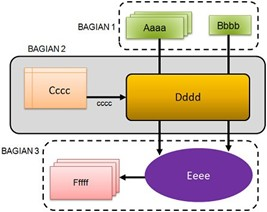
\includegraphics[width=0.6\textwidth]{gambar_desain_sistem.jpeg}
  \caption{Desain sistem dari solusi yang ditawarkan}
  \label{fig:desain_sistem}
\end{figure}

% ── Contoh gambar dengan sumber kutipan ──────────────────────
% Sumber dicantumkan di bawah gambar, di atas caption, ukuran 11pt
\begin{figure}[H]
  \centering
  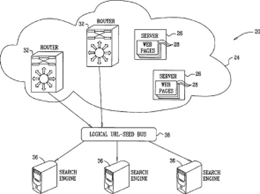
\includegraphics[width=0.6\textwidth]{gambar_kutipan.png}

  \vspace{4pt}
  {\fontsize{12}{15}\selectfont\itshape Sumber: http://alamat-sumber.com/gambar.jpg\par}

  \caption{Contoh gambar kutipan}
  \label{fig:gambar_kutipan}
\end{figure}

\subsection{Bagian 1}

Disini penulis dapat menjelaskan lebih terperinci apa saja yang ada pada bagian
ini. Jika bagian ini mempunyai sub bagian yang perlu diperjelas dalam
pembahasan, penulis dapat menuliskannya dalam sub pembahasan pada bagian ini.

\subsubsection{Aaaa}

Disini penulis dapat membahas sub bagian Aaaa lebih terperinci. Deskripsi
pembahasan seharusnya singkat, padat dan jelas, sehingga membuat pembaca
memahami maksud penulis yang tertuang dalam tulisan. Apabila pembahasan penulis
memerlukan penulisan persamaan matematis, penulis dapat menuliskannya seperti
pada Persamaan~\ref{eq:binomial}.

\begin{equation}
  (x+a)^n = \sum_{k=0}^{n} \binom{n}{k} x^k a^{n-k}
  \label{eq:binomial}
\end{equation}

Persamaan~\ref{eq:binomial} menunjukkan teorema binomial yang merupakan dasar dari
metode yang digunakan.

% ── Contoh tabel dengan sumber kutipan (tabularray) ──────────
\begin{table}[H]
  \centering
  \caption{Contoh penulisan tabel otomatis}
  \label{tab:contoh1}
  \begin{tblr}{colspec={c c c}}
    Kolom 1  & Kolom 2  & Kolom 3  \\
    Data 1-1 & Data 1-2 & Data 1-3 \\
    Data 2-1 & Data 2-2 & Data 2-3 \\
  \end{tblr}

  \vspace{4pt}
  {\fontsize{12}{15}\selectfont Sumber: Badan Pusat Pengolahan Data, 2026 \cite{buku_contoh}\par}
\end{table}

\subsection{Bagian 2}

Disini penulis dapat menjelaskan lebih terperinci apa saja yang ada pada Bagian 2 ini.
Deskripsi pembahasan seharusnya singkat, padat, dan jelas sehingga membuat pembaca
memahami maksud penulis yang tertuang dalam tulisan.

% ── Contoh tabel biasa tanpa sumber (tabularray) ─────────────
\begin{table}[H]
  \centering
  \caption{Contoh penulisan tabel 2}
  \label{tab:contoh2}
  \begin{tblr}{colspec={c c c c}}
    Kolom 1 & Kolom 2 & Kolom 3 & Kolom 4 \\
    Data 1-1 & Data 1-2 & Data 1-3 & Data 1-4 \\
    Data 2-1 & Data 2-2 & Data 2-3 & Data 2-4 \\
  \end{tblr}
\end{table}

\begin{equation}
  F = m \cdot a
  \label{eq:newton}
\end{equation}

\subsection{Bagian 3}

Disini penulis dapat menjelaskan lebih terperinci apa saja yang ada pada Bagian 3 ini.
Deskripsi pembahasan seharusnya singkat, padat, dan jelas sehingga membuat pembaca
memahami maksud penulis yang tertuang dalam tulisan.

\begin{equation}
  \lim_{x \to c} f(x) = L
  \label{eq:limit}
\end{equation}

% Daftar Pustaka
\ifshowforceoddpage\cleartooddpage\else\clearpage\fi
\addcontentsline{toc}{chapter}{DAFTAR PUSTAKA}
\renewcommand{\bibname}{DAFTAR PUSTAKA}
\bibliographystyle{refs/IEEEtranN}
\bibliography{refs/references}

%============================================================
\end{document}
%============================================================
